%%%%%%%%%%%%%%%%%%%%%%%%%%%%%%%%%%%%%%%%%
% Jacobs Landscape Poster
% LaTeX Template
% Version 1.1 (14/06/14)
%
% Created by:
% Computational Physics and Biophysics Group, Jacobs University
% https://teamwork.jacobs-university.de:8443/confluence/display/CoPandBiG/LaTeX+Poster
% 
% Further modified by:
% Nathaniel Johnston (nathaniel@njohnston.ca)
%
% This template has been downloaded from:
% http://www.LaTeXTemplates.com
%
% License:
% CC BY-NC-SA 3.0 (http://creativecommons.org/licenses/by-nc-sa/3.0/)
%
%%%%%%%%%%%%%%%%%%%%%%%%%%%%%%%%%%%%%%%%%

%----------------------------------------------------------------------------------------
%	PACKAGES AND OTHER DOCUMENT CONFIGURATIONS
%----------------------------------------------------------------------------------------

\documentclass[final]{beamer}

\usepackage{etex}
\usepackage[scale=1.24]{beamerposter} % Use the beamerposter package for laying out the poster

\usetheme{confposter} % Use the confposter theme supplied with this template

\setbeamercolor{block title}{fg=Triad-Blue,bg=white} % Colors of the block titles
\setbeamercolor{block body}{fg=black,bg=white} % Colors of the body of blocks
\setbeamercolor{block alerted title}{fg=white,bg=Stanford!70} % Colors of the highlighted block titles
\setbeamercolor{block alerted body}{fg=black,bg=Stanford!10} % Colors of the body of highlighted blocks
% Many more colors are available for use in beamerthemeconfposter.sty

%-----------------------------------------------------------
% Define the column widths and overall poster size
% To set effective sepwid, onecolwid and twocolwid values, first choose how many columns you want and how much separation you want between columns
% In this template, the separation width chosen is 0.024 of the paper width and a 4-column layout
% onecolwid should therefore be (1-(# of columns+1)*sepwid)/# of columns e.g. (1-(4+1)*0.024)/4 = 0.22
% Set twocolwid to be (2*onecolwid)+sepwid = 0.464
% Set threecolwid to be (3*onecolwid)+2*sepwid = 0.708

\newlength{\sepwid}
\newlength{\onecolwid}
\newlength{\twocolwid}
\newlength{\threecolwid}
\setlength{\paperwidth}{48in} % A0 width: 46.8in
\setlength{\paperheight}{36in} % A0 height: 33.1in
\setlength{\sepwid}{0.024\paperwidth} % Separation width (white space) between columns
\setlength{\onecolwid}{0.22\paperwidth} % Width of one column
\setlength{\twocolwid}{0.464\paperwidth} % Width of two columns
\setlength{\threecolwid}{0.708\paperwidth} % Width of three columns
\setlength{\topmargin}{-0.5in} % Reduce the top margin size
%-----------------------------------------------------------

\usepackage{graphicx}

\usepackage{booktabs} % Top and bottom rules for tables

\usepackage{phonetic}
\usepackage{tipa}
\usepackage[normalem]{ulem}
\usepackage{pifont}
\usepackage{gb4e}
\usepackage{apacite}
\usepackage[round]{natbib}
\usepackage{bibentry}
\usepackage[nocenter]{qtree}
\usepackage{pst-tree}
\usepackage{multicol}
\usepackage{multirow}

\newcommand\barh{\ipabar{h}{1.1ex}{.6}{}{.3}}
\renewcommand{\rmdefault}{ptm}

\renewcommand*{\bibfont}{\scriptsize}

%----------------------------------------------------------------------------------------
%	TITLE SECTION 
%----------------------------------------------------------------------------------------

\title{Agreement in English Existentials with Conjoined Associates} % Poster title

\author{Phil Crone \& Bonnie Krejci | Stanford University} % Author(s)

% \institute{} % Institution(s)

%----------------------------------------------------------------------------------------

\begin{document}

\addtobeamertemplate{block end}{}{\vspace*{2ex}} % White space under blocks
\addtobeamertemplate{block alerted end}{}{\vspace*{2ex}} % White space under highlighted (alert) blocks

\setlength{\belowcaptionskip}{2ex} % White space under figures
\setlength\belowdisplayshortskip{2ex} % White space under equations

\begin{frame}[t] % The whole poster is enclosed in one beamer frame

\begin{columns}[t] % The whole poster consists of four columns.

\begin{column}{\sepwid}\end{column} % Empty spacer column

\begin{column}{\onecolwid} % The first column

\vspace{-0.25em} \begin{block}{Explananda} \vspace{0.5em}

English existential clauses have notoriously unexpected agreement patterns, more so when the associate is conjoined~\citep{Chomsky95, Sobin97, Sobin14, Schutze99}. 

\begin{exe}

\ex\label{variation} \textsc{Agreement Variation with No Conjunction}
	\begin{xlist}
	\ex[\%]{\textcolor{Triad-Yellow}{There is basically \textbf{no jobs} in industry.}} \label{singular-non-conj}
	\ex[]{\label{there's} There's \textbf{only two thrift shops} down there.} 
	\ex[]{\label{standard-pl} There are \textbf{more new subdivisions} in town.}
	\end{xlist}

\ex\label{singular} \textsc{Singular Agreement with Conjunction:}
	\begin{xlist}
	\ex[\%]{\textcolor{Triad-Blue}{There is \textbf{[[conversations] and [rhetoric]]}}}\label{singular-conj}
	\ex[]{\label{singular-conj-sg} \textcolor{Stanford}{There is \textbf{[[a prominent actor] and [actress]]}}}
	\end{xlist}

\ex\label{plural} \textsc{Plural Agreement with Conjunction:}
	\begin{xlist}
	\ex[]{\label{plural-conj-sg} There are \textbf{[[Bluebeard] and [Henry VIII]]}}
	\ex[]{\label{plural-conj-pl} There are \textbf{enough  [[actors] and [actresses]]}}
	\end{xlist}
\end{exe}

\end{block}

\begin{alertblock}{Claims}
\begin{itemize}
\item The pattern in  (\ref{singular-conj-sg}) is a case of First Conjunct Agreement (FCA) and should be analyzed in the same way as FCA in other languages.
\item This pattern is not reducible to the fact that a singular verb form is possible with a plural associate (i.e., that (\ref{singular-non-conj}) and (\ref{singular-conj}) are possible). 
\end{itemize}

\end{alertblock}

\begin{block}{First Conjunct Agreement}\vspace{0.5em}

In many languages, verbs may agree with either the first conjunct of a conjoined subject DP or the full conjunction when the subject appears post-verbally.
\begin{exe}
    \ex Lebanese Arabic \citep{Aoun:1994}
\vspace{-.5em}
    \gll \textbf{raa{\barh}}/\textbf{raa\barh-o} [Kariim w Marwaan].\\
        \textbf{left.\textsc{3msg}/-\textsc{3pl}} Kareem and Marwan\\
\vspace{-.5em}
        \trans ``Kareem and Marwan left.''
    \ex Colloquial Finnish \citep[85-86]{vanKoppen:2005}
\vspace{-.5em} \gll sit\"{a} \textbf{ole-n/-mme} [min\"{a} ja sin\"{a}-kin] k\"{a}y-neet Pariisi-ssa.\\
        \textsc{expl} \textbf{be-\textsc{1sg}/-\textsc{1pl}} I and you-also visit-\textsc{ptc.pl} Paris-\textsc{ine}\\
\vspace{-.5em}
        \trans ``You and I have visited Paris.''
\end{exe}
We account for FCA as follows:
\begin{itemize}
    \item Assume standard definition of Agree (Chomsky, 2000; 2004) and asymmetrical structure of conjunction \citep{Munn:1993,Kayne94,Zoerner:1995}.
    \item When a \(\varphi\)-probe c-commands a conjoined subject DP, neither the first conjunct nor full conjunction c-commands the other; both are potential goals for Agree.
\end{itemize}
\begin{exe}
\ex \Tree [.TP [.{\rnode{T}{T \([u\varphi]\)}} ] [.{\ldots} [.{\rnode{DP1}{DP \([\varphi]\)}} [.{\rnode{DP2}{DP \([\varphi]\)}} ] [ [.{\&} ] [.{DP \([\varphi]\)} ] ] ] [.{\ldots} ] ] ]
    	\nccurve[linestyle=dotted,linewidth=0.1em,angleA=-45,angleB=180,nodesep=0.1]{->}{T}{DP1}
		\naput{\(\varphi\)}
		\nccurve[linestyle=dotted,linewidth=0.1em,angleA=-90,angleB=180,nodesep=0.1]{->}{T}{DP2}
		\nbput{\(\varphi\)}
\end{exe}

\end{block}

\end{column} % End of the first column

\begin{column}{\sepwid}\end{column} % Empty spacer column

\begin{column}{\twocolwid} % Begin a column which is two columns wide (column 2)

\begin{columns}[t,totalwidth=\twocolwid] % Split up the two columns wide column

\begin{column}{\onecolwid}\vspace{-.6in} % The first column within column 2 (column 2.1)

\begin{block}{Proposal}\vspace{0.5em}
Structure of \textit{there} existentials \citep[see][i.a.]{Chomsky95, Sobin97, Schutze99, Richards05, Rezac06, Deal09, Sobin14}:
\begin{exe}
\ex \Tree [.TP [.There ] [ [.\rnode{T}{T [\(u\varphi\)]} ] [.{\ldots} [.be ] [.{\ldots} [.\rnode{DP1}{DP [\(\varphi\)]} [.\rnode{DP2}{DP [\(\varphi\)]} ] [ [.\& ] [.{DP [\(\varphi\)]} ] ] ] [.{\ldots} ] ] ] ] ]
        \nccurve[linestyle=dotted,linewidth=0.1em,angleA=-90,angleB=180,nodesep=0.1]{->}{T}{DP1}
		\nbput{\(\varphi\)}
		\nccurve[linestyle=dotted,linewidth=0.1em,angleA=-135,angleB=180,nodesep=0.1]{->}{T}{DP2}
		\nbput{\(\varphi\)}
\end{exe}
In this configuration, T may Agree with either the full conjunction or the first conjunct of the associate DP.
\end{block}

\begin{block}{FCA vs. Non-Standard Singular Agreement}\vspace{0.5em}
Alternatively, we might explain (\ref{singular-conj-sg}) in virtue of the fact that singular agreement is possible in existential constructions with plural associates more generally (\ref{singular-non-conj}, \ref{singular-conj}). However:
\begin{itemize}
\item (\ref{singular-conj-sg}) is cited as standard English \citep[e.g.,][]{Sobin14}, whereas examples like (\ref{singular-non-conj}) pattern in usage and perception like non-standard morphosyntactic variables (\citealt{Krejci:2015,Hilton:2015}).
\item Data from COCA show that the pattern in (\ref{singular-conj-sg}) is used much more frequently than that in (\ref{singular-non-conj}) or  (\ref{singular-conj}).
\end{itemize}

\setlength{\tabcolsep}{3pt}
\begin{center}
\begin{tabular}{| c | c | c | c | c |}
\hline
 & \multicolumn{2}{| c |}{Singular First Conjunct} & \multicolumn{2}{| c |}{Plural First Conjunct} \\
\hline
 \textit{is/has been} & \textcolor{Stanford}{\textbf{1,097 (48.4\%)}} & {2,211} & \textcolor{Triad-Blue}{\textbf{22 (1.1\%)}} & {187}\\
 \cline{1-2}\cline{4-4}
\textit{'s/'s been} & 1,114 (49.1\%) & (97.5\%) & 165 (8.4\%) & (9.5\%) \\
\hline
\textit{are/have been} & \multicolumn{2}{|c|}{56 (2.5\%)} & \multicolumn{2}{|c|}{1,780 (90.5\%)}\\
\hline
\end{tabular}
\end{center}

\setlength{\tabcolsep}{3pt}
\begin{center}
\begin{tabular}{| c | c | c | c | c |}
\hline
 & \multicolumn{2}{| c |}{Singular Non-conjoined} & \multicolumn{2}{| c |}{Plural Non-conjoined} \\
\hline
 \textit{is/has been} & 86,322 (46.0\%) & {184,363} & \textcolor{Triad-Yellow}{\textbf{642 (1.0\%)}} & {5,640}\\
 \cline{1-2}\cline{4-4}
\textit{'s/'s been} & 98,041 (52.3\%) & (98.3\%) & 4,998 (7.5\%) & (8.5\%) \\
\hline
\textit{are/have been} & \multicolumn{2}{|c|}{3,238 (1.7\%)} & \multicolumn{2}{|c|}{60,696 (91.5\%)}\\
\hline
\end{tabular}
\end{center}

\begin{itemize}
\item Acceptability judgments from native speakers (\(N = 47\)) show the pattern in (\ref{singular-conj-sg}) to be much more acceptable than the patterns in (\ref{singular-non-conj}) and  (\ref{singular-conj}).
\end{itemize}
\vspace{1em}
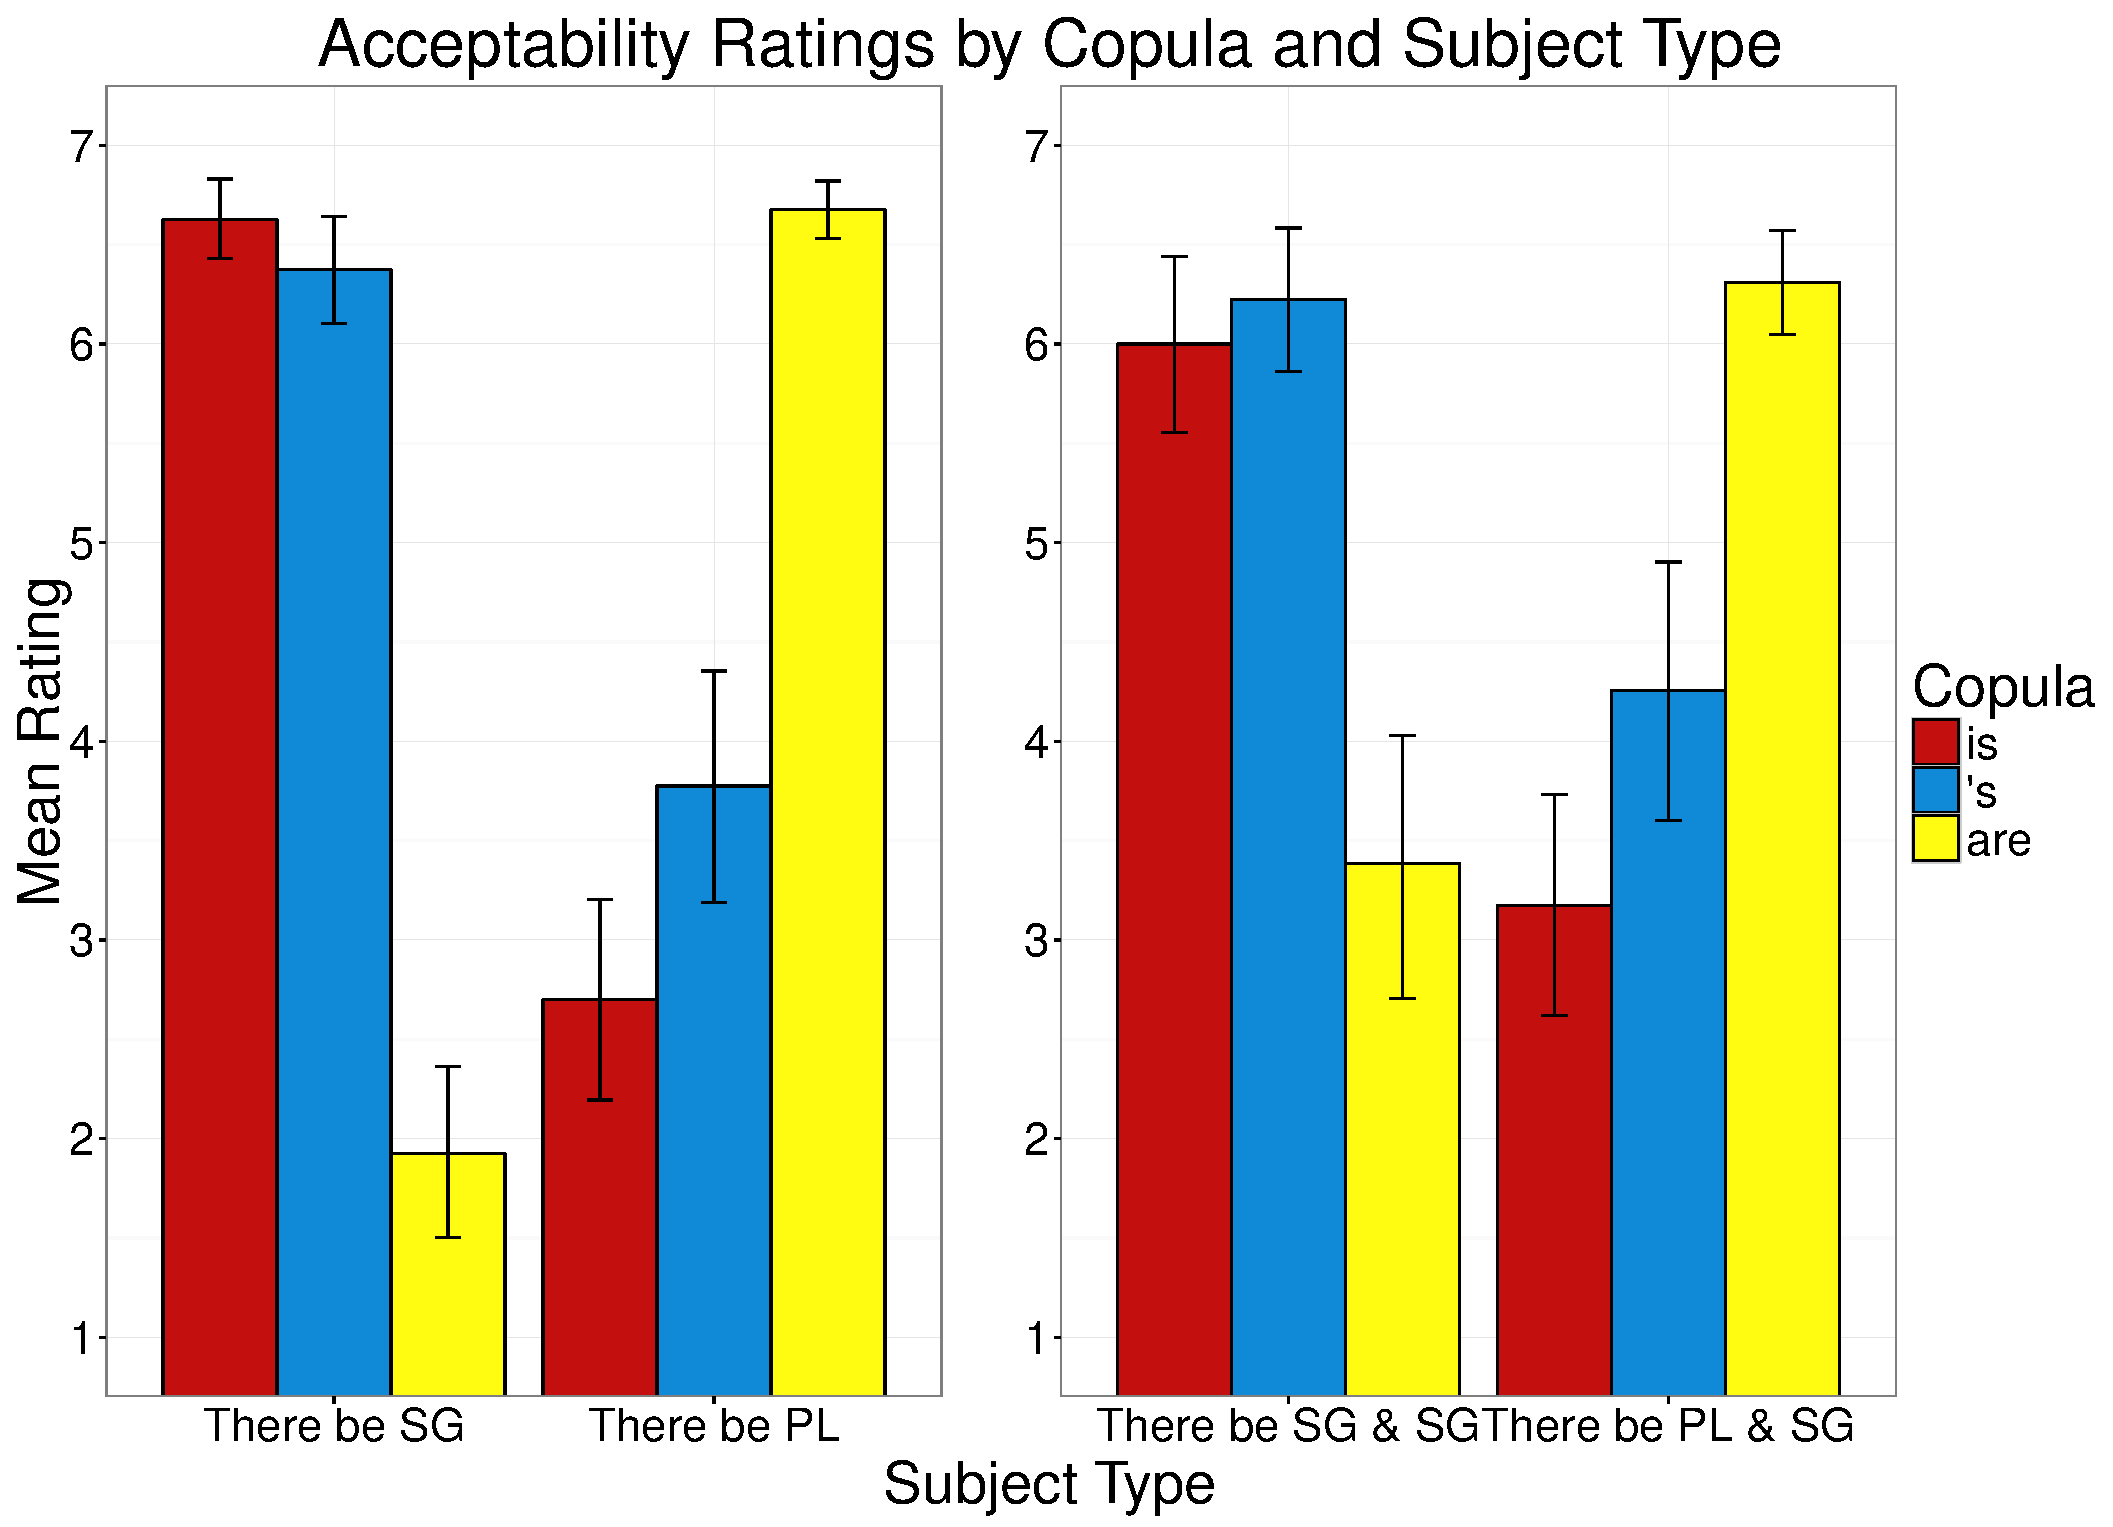
\includegraphics[width=\onecolwid]{Plot-color.eps}

\end{block}

\end{column} % End of column 2.1

\begin{column}{\onecolwid}\vspace{-.6in} % The second column within column 2 (column 2.2)

\begin{block}{Ellipsis}\vspace{0.5em}
Sentence (\ref{singular-conj-sg}) could be an instance of ellipsis: \textit{there is an actor and [\sout{there is}] an actress}.
\begin{itemize}
\item This would require ellipsis to target a non-constituent.
\item This analysis is inconsistent with \textit{there} existentials that contain predicates requiring plural subjects:
\begin{exe}
\ex\label{ellipsis-full1} \# There is a professor meeting together and there is a student meeting together.
\ex\label{ellipsis-elided} There is a professor and a student meeting together.
\end{exe}

\end{itemize}
\end{block}

\begin{block}{FCA: Hierarchical or Linear?}\vspace{0.5em}
\cite{Sobin14} generates (\ref{singular-conj-sg}) by having T search linearly for the nearest lexical DP with which to agree. However:
\begin{itemize}
\item Agree usually operates hierarchically; it is unexplained why it would operate linearly for only conjoined associate DPs.
\item Examples such as (\ref{plural-conj-sg}) are not generated.
\item This analysis faces difficulties in explaining obligatory full agreement with pre-verbal, conjoined subjects. 
\end{itemize}\vspace{-0.5em}
\begin{exe}
\ex{John and Mary are/*is tired.}\label{english-preverbal}
\ex \label{la-preverbal} Lebanese Arabic \citep{Aoun:1994}
\vspace{-.5em}
 \gll [Kariim w Marwaan] \textbf{raa\barh-o}/*\textbf{raa{\barh}}.\\
    Kareem and Marwan \textbf{left-\textsc{3pl}}/*\textbf{left.\textsc{3ms}}\\
    \vspace{-.5em}
    \trans ``Kareem and Marwan left.''
    \ex \label{finnish-preverbal} Colloquial Finnish \citep[85-86]{vanKoppen:2005}
\vspace{-.5em}
    \gll [min\"{a} ja sin\"{a}-kin] sit\"{a} \textbf{ole-mme}/*\textbf{-n}/*-\textbf{t} k\"{a}y-neet Pariisi-ssa.\\
    I and you-also \textsc{expl} \textbf{be-\textsc{1pl}}/*\textbf{-\textsc{1sg}}/*\textbf{-\textsc{2sg}} visit-\textsc{ptc.pl} Paris-\textsc{ine}\\
    \vspace{-.5em}
    \trans ``You and I have visited Paris.''
\end{exe}\vspace{-0.5em}
\begin{itemize}
\item Two ways to account for data in (\ref{english-preverbal}) - (\ref{finnish-preverbal}) hierarchically: interaction between constraints on Agree and movement \citep{Doron:2000,vanKoppen:2012,Crone:2015}, as in (\ref{movement}), or bidirectional Agree \citep{Baker:2008}, as in (\ref{bidirection}).
\end{itemize}
\begin{exe}
\ex \label{movement} \Tree [.TP [.{\rnode{Spec-TP}{DP}} ] [ [.{\rnode{T}{T \([u\varphi]\)}} ] [.{\ldots} [.{\rnode{DP1}{DP \([\varphi]\)}} [.{DP\([\varphi]\)} ] [ [.{\&} ] [.{DP\([\varphi]\)} ] ] ] [.{\ldots} ] ] ] ]
		\nccurve[linestyle=dotted,linewidth=0.1em,angleA=-45,angleB=180,nodesep=0.1]{->}{T}{DP1}
		\naput{\(\varphi\)}
		\nccurve[linewidth=0.1em,angleA=-135,angleB=-90,nodesep=0.1,ncurv=0.75]{->}{DP1}{Spec-TP}
\ex \label{bidirection} \Tree [.TP [.{\rnode{DP1}{DP \([\varphi]\)}} [.{\rnode{DP2}{DP \([\varphi]\)}} ] [ [.{\&} ] [.{DP\([\varphi]\)} ] ] ] [ [.{\rnode{T}{T \([u\varphi]\)}} ] [.{\ldots} ] ] ]
		\nccurve[linestyle=dotted,linewidth=0.1em,angleA=-180,angleB=0,nodesep=0.1]{->}{T}{DP1}
		\nbput{\(\varphi\)}
		\nccurve[linestyle=dotted,linewidth=0.1em,angleA=-90,angleB=-90,nodesep=0.1]{->}{T}{DP2}
		\ncput{\ding{55}}
\end{exe}\vspace{0.5em}
\begin{itemize}
\item If agreement is linear regardless of whether the subject is pre- or post-verbal, last conjunct agreement (LCA) with pre-verbal subjects is predicted.
\item Therefore, this account must stipulate that agreement is linear only for post-verbal subjects.
\end{itemize}

\end{block}


\end{column} % End of column 2.2

\end{columns}

\end{column}

\begin{column}{\sepwid}\end{column} % Empty spacer column

\begin{column}{\onecolwid} % The third column

\vspace{-0.25em} \begin{block}{Outstanding Questions} \vspace{0.5em}

Why is full agreement less acceptable than FCA? We offer no explanation, but note similar phenomena in other languages:
\begin{itemize}
\item \textbf{Tegelen Dutch}: Complementizers obligatorily realize FCA unless some element intervenes between the complementizer and the subject (\citealt{vanKoppen:2012}).
\item \textbf{Biblical Hebrew}: Both FCA and full agreement are attested in VS clauses, but FCA occurs in 210 of 235 (89.4\%) clauses with post-verbal conjoined subjects (\citealt{Moreshet:1967, Doron:2000}).
\end{itemize}
Where else do we predict to see FCA in English?
\begin{itemize}
\item The possibility of FCA depends on the relative position of the subject DP with respect to T, not the positions of the subject and the verb. 
\item If a verb raises to C and the subject DP occupies [Spec, TP], we do not predict FCA to be possible.
\end{itemize}
\begin{center}
    \begin{tabular}{ll}
    Phenomenon & FCA Possible? \\
    \hline
    Questions & No\\
    Residual V2 & No \\
    Locative inversion & Maybe (depends on analysis of LI)
    \end{tabular}
\end{center}

\end{block}

\begin{block}{Selected References}

\bibliographystyle{apalike}
\bibliography{References}
\end{block}

\begin{block}{Acknowledgments}\vspace{0.5em}
\small{The authors gratefully acknowledge Vera Gribanova, Arto Anttila, Chris Manning, Boris Harizanov, Beth Levin, Paul Kiparsky, and John Rickford for their support and feedback on this project. We also thank the Stanford Syntax Morphology Circle for their helpful comments on earlier versions of this work, as well as Penny Eckert and the contributors to the Voices of California Project.} \\

\end{block}

%----------------------------------------------------------------------------------------
%	CONTACT INFORMATION
%----------------------------------------------------------------------------------------

\begin{alertblock}{Contact Information}

\textsc{Phil Crone}: \texttt{pcrone@stanford.edu}

\textsc{Bonnie Krejci}: \texttt{bkrejci@stanford.edu}

\end{alertblock}

\end{column} % End of the third column

\end{columns} % End of all the columns in the poster

\end{frame} % End of the enclosing frame

\end{document}